\chapter{System build and estimation}
\label{ch:estimate}

The two techniques are estimated on a numerical plant that is the same plant the design equations describe. Section~\ref{sec:build} records the build: the algebraic header, the sticky positioners, the transmitters, the analyser, and the three controllers that are compared. Section~\ref{sec:estimation} records the campaign and reads the extract error, the beer-flow error and the valve travel. The campaign is not a factory trial. It is a controlled estimation in which every disturbance is known and every controller sees the same noise sequence, so that differences can be attributed to the control law.

\section{System build}
\label{sec:build}

\subsection{Numerical plant}

The plant state is the three stems. Everything else is algebraic or is a filter on a measurement. At each step of \SI{10}{ms} the following is computed, in order.

The boundary pressures and the external setpoints are set by the scenario clock of Section~\ref{sec:estimation}. The beer-valve coefficient is the design $K_{v,h}$ until \SI{480}{s} and ninety percent of that value afterwards. Header pressure is the unique root of \eqref{eq:node}. With that pressure, \eqref{eq:kv} gives the three flows, the speeds follow from the pipe areas, and \eqref{eq:plato-vol} with the true mother-beer extract gives the true original extract at the mix point. The true extract is not shown to any controller. It is the quantity whose error is integrated at the end.

Transmitters add independent Gaussian noise and a \SI{0.30}{s} lag. The standard deviations are \SI{0.012}{\cubic\metre\per\hour} on beer flow, \SI{0.006}{\cubic\metre\per\hour} on water flow, \SI{0.0035}{\barg} on header pressure, \SI{0.0015}{stem fraction} on each position, and \SI{0.006}{\plato} on the analyser. These figures sit inside the accuracy of a sanitary magnetic flowmeter and a sanitary pressure transmitter \cite{baker2016flow,liptak2006handbook}. The same random draw is used for every controller, so a noise spike is not credited to one of them.

The analyser buffer stores the true extract. The value delayed by the current $\tau_d$ is passed through \eqref{eq:analyser}. Because $\tau_d$ depends on $v_b$, a throughput change stretches or compresses the delay during the run. At the design speed $\tau_d=\SI{9.86}{s}$. At the high rate the outlet speed rises and the delay falls toward \SI{8}{s}. The soft-sensor bias uses the same stretch, which is Assumption~\ref{as:delay-known} implemented literally.

Positioners obey \eqref{eq:exact-pos} and the stick rule of Section~\ref{sec:tech1}. A command filter of \SI{0.40}{s} is placed in front of every positioner for every controller. It represents the filtering a positioner already applies, and it prevents a comparison from rewarding a law that chatters the command inside the stick band.

The build was checked at $t=0$ with the design commands. The solved header pressure is \SI{2.40}{\barg}, the three flows match Table~\ref{tab:design} to three decimals, the extract is \SI{12.000}{\plato}, and the installed gains match \eqref{eq:Gdesign}. A separate check steps the beer command by $0.1$ with the other commands held and confirms that the initial derivative of $Q_h$ equals $b_{0,h}\times 0.1$. Those two checks are the build acceptance tests. A controller comparison on a plant that failed them would not be an estimation of the design.

\subsection{The three controllers}

Three controllers are built on this plant.

The first is ratio proportional--integral control, the industrial baseline \cite{shinskey1996process,skogestad2003simc,seborg2016process}. Each loop is in velocity form so that an output limit stops the integration instead of winding it \cite{astrom2006advanced}. The beer and water flow gains follow SIMC at the design installed gains with a closed-loop time constant of $1.15\tau_v$:
\begin{equation}
K_{p,h} = \frac{\tau_v}{G_{hh}\times 1.15} = 0.272, \qquad T_{i,h} = \tau_v = \SI{2.4}{s},
\end{equation}
and $K_{p,w} = 0.516$ with the same integral time. The header loop uses the positive gain
\begin{equation}
K_{p,m} = \frac{\tau_v}{|G_{bp}|\times 3.5} = 0.150, \qquad T_{i,m} = \SI{8}{s},
\end{equation}
and a fixed setpoint of \SI{2.40}{\barg}. The sign is arranged so that a high header opens the outlet valve. The extract loop trims $R$ from $P_{\mathrm{meas}}$ only, with $K_R = -0.00884$ and integral time \SI{22}{s}, the delay-dominated SIMC setting of Section~\ref{sec:tech2}. The water setpoint is $R Q_h^\star$.

The second controller is linear active disturbance rejection with the gains frozen at the design point \cite{gao2003scaling,han2009pid}. The flow observers use \eqref{eq:flow-bw} and $b_{0,h}=3.195$, $b_{0,w}=1.684$, with no update when the pressures move. The header observer uses \eqref{eq:p-bw} and $b_{0,p}=-1.910$, and it holds \SI{2.40}{\barg}. The extract observer uses $\omega_{c,R}=0.055$, $\omega_{o,R}=0.22$ and $b_{0,R}=-4.038$, and its feedback is $P_{\mathrm{meas}}$. This controller has the same flow bandwidth and the same header bandwidth as the proposed controller. The differences are the frozen gains, the fixed header setpoint, and the delayed extract feedback. Those are the three differences the estimation is intended to isolate.

The third controller is the pair designed in Chapter~\ref{ch:design}. Installed gains are computed from the filtered measurements by \eqref{eq:Ghh}--\eqref{eq:Gbp}, filtered over \SI{2.5}{s}, and corrected by \eqref{eq:z2-invariance}. The header setpoint minimises \eqref{eq:cost}. The extract feedback is \eqref{eq:pctrl}. Bandwidths are Table~\ref{tab:bw}.

All three start at the design stems, with observer states at the consistent values \eqref{eq:z2init}. The first \SI{50}{s} of the campaign are therefore a test that the initialisation and the noise do not themselves leave the extract tolerance. They do not: the integrated absolute extract error of each controller over \SIrange{10}{50}{s} is $0.005\degP\cdot\mathrm{s}$, which is the analyser noise floor, and the valve travel in that window is zero because the stick bands hold the stems.

\subsection{Scenario clock}

One run lasts \SI{560}{s} and contains the six disturbances of Section~\ref{sec:problem}, in an order that lets each transient be seen before the next begins. Table~\ref{tab:clock} is the clock. The pressure step is a true step. The brand change, the throughput change and the mother-beer drift are ramps, because an operator does not step a beer setpoint \cite{kunze2014brewing,shinskey1996process}. The loss of $K_v$ is a step, because a piece of fouling does not announce itself with a ramp.

\begin{table}[htbp]
\centering
\caption{Scenario clock.}
\label{tab:clock}
\begin{tabular}{@{}llp{7.2cm}@{}}
\toprule
Time (s) & Name & Action \\
\midrule
0--50 & steady & Design point, measurement noise only \\
50 & pressure step & Beer supply from \SI{4.00}{\barg} to \SI{3.05}{\barg}, held thereafter \\
130--210 & water oscillation & Water supply $4.20+0.28\sin(2\pi t/26)$ \\
230--255 & brand change & $P^\star$ ramped from \SI{12.0}{\plato} to \SI{11.2}{\plato} \\
320--340 & throughput & $Q_h^\star$ ramped from 7.50 to \SI{9.00}{\cubic\metre\per\hour} \\
400--440 & extract drift & True $P_h$ ramped from 16.0 to \SI{16.6}{\plato}, hidden from the controllers \\
480 & valve wear & Beer $K_v$ multiplied by 0.90, hidden from the controllers \\
\bottomrule
\end{tabular}
\end{table}

\subsection{Indices}

Three indices are computed on each window and on the full run. The integrated absolute extract error is
\begin{equation}
\label{eq:iae}
\mathrm{IAE} = \int_{t_0}^{t_1} \big|P(t)-P^\star(t)\big|\,\ud t,
\end{equation}
in $\degP\cdot\mathrm{s}$, using the true mix-point extract. The integrated absolute beer-flow error is the same integral on $Q_h-Q_h^\star$, in $\si{\cubic\metre\per\hour\second}$. Valve travel is the sum of absolute stem increments, a dimensionless measure of how far the positioner moved. A controller that holds the extract by a large travel may still be unacceptable if the travel is a high-frequency chatter inside the stick band; the travel figures below are inspected against the stem plots for that failure. Settling time is the last instant in the window at which the extract error exceeds \SI{0.05}{\plato}, measured from the start of the window. A window in which the error never re-enters the band has no settling time.

The instantaneous extract error at the pressure step is about \SI{1.0}{\plato} for every controller. The beer flow depends algebraically on $p_h$, so the flow, and therefore the extract, jumps in the sample of the step, before any positioner has moved. That jump is a property of the plant. The indices that discriminate the controllers are the integral after the jump and the settling time.

\section{Estimation}
\label{sec:estimation}

\subsection{Overall comparison}

Table~\ref{tab:overall} gives the full-run indices. Figure~\ref{fig:iae} shows the extract integral window by window. Figure~\ref{fig:plato} shows the true extract against its setpoint, and Figure~\ref{fig:zoom} shows the pressure step and the brand change at a scale where the tolerance band is visible.

\begin{table}[htbp]
\centering
\caption{Full-run indices, \SIrange{0}{560}{s}.}
\label{tab:overall}
\begin{tabular}{@{}lrrr@{}}
\toprule
Index & PID ratio & Fixed-gain LADRC & Proposed \\
\midrule
Extract IAE ($\degP\cdot\mathrm{s}$) & 524 & 81.4 & 52.4 \\
Beer-flow IAE (\si{\cubic\metre\per\hour\second}) & 286 & 316 & 37.5 \\
Time outside $\pm 0.05\degP$ (s) & 384 & 333 & 271 \\
Beer-valve travel & 2.99 & 5.93 & 7.02 \\
Water-valve travel & 2.33 & 3.86 & 5.14 \\
Outlet-valve travel & 0.61 & 1.41 & 3.44 \\
\bottomrule
\end{tabular}
\end{table}

The extract integral of the proposed pair is $64$ percent of the fixed-gain active-disturbance-rejection integral and one tenth of the proportional--integral integral. The beer-flow integral is about one eighth of either baseline. The baselines spend that flow error at the open stop: after the supply step their beer stems sit between $0.90$ and $0.98$ and never recover the \SI{9}{\cubic\metre\per\hour} demand. The proposed beer stem is at $0.77$ at the end of the run, the water stem at $0.75$ and the outlet stem at $0.73$, and the beer flow is \SI{9.06}{\cubic\metre\per\hour} against a setpoint of \SI{9.00}{\cubic\metre\per\hour}.

The extra outlet travel, $3.44$ against $1.41$ and $0.61$, is the coordinator doing the work the baselines do not do. It is not chatter. Figure~\ref{fig:valves} shows three slow moves, at the supply step, at the throughput ramp and at the $K_v$ loss, rather than a filled band of noise. The shaded band on that figure is the linear window used by \eqref{eq:schedule}. The proposed stems leave it only briefly. The baseline beer stems enter it at the start and do not return.

\begin{figure}[htbp]
\centering
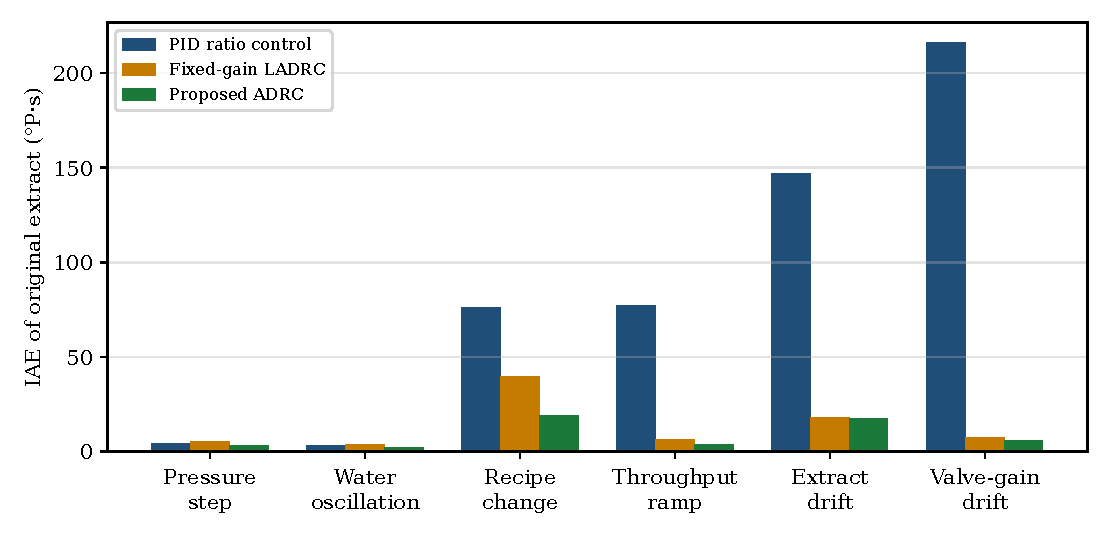
\includegraphics[width=\textwidth]{iae_bars.pdf}
\caption{Integrated absolute error of original extract on each disturbance window.}
\label{fig:iae}
\end{figure}

\begin{figure}[htbp]
\centering
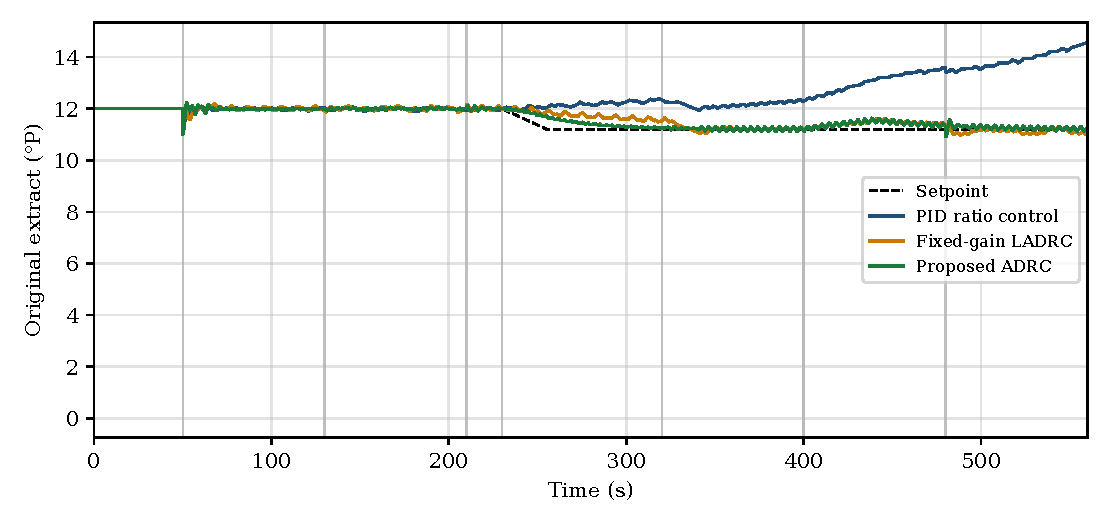
\includegraphics[width=\textwidth]{plato_full.pdf}
\caption{True original extract over the campaign. Vertical lines mark the events of Table~\ref{tab:clock}.}
\label{fig:plato}
\end{figure}

\begin{figure}[htbp]
\centering
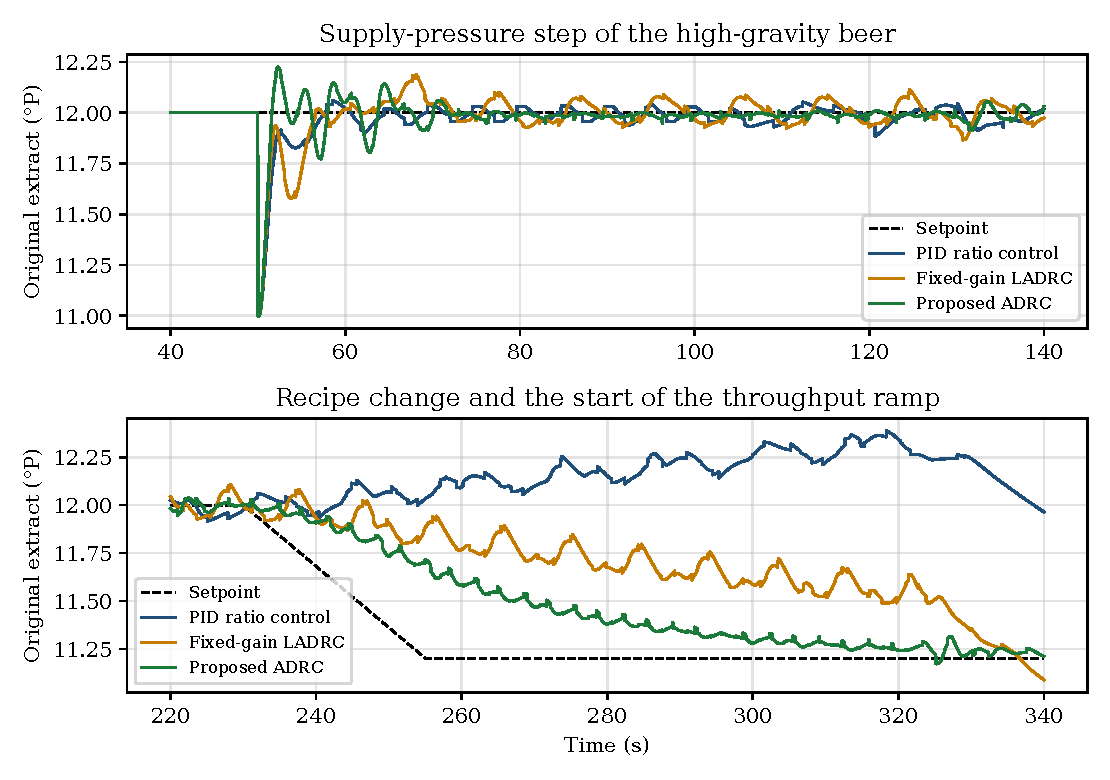
\includegraphics[width=\textwidth]{plato_zoom.pdf}
\caption{Original extract during the beer-supply step and during the brand change.}
\label{fig:zoom}
\end{figure}

\begin{figure}[htbp]
\centering
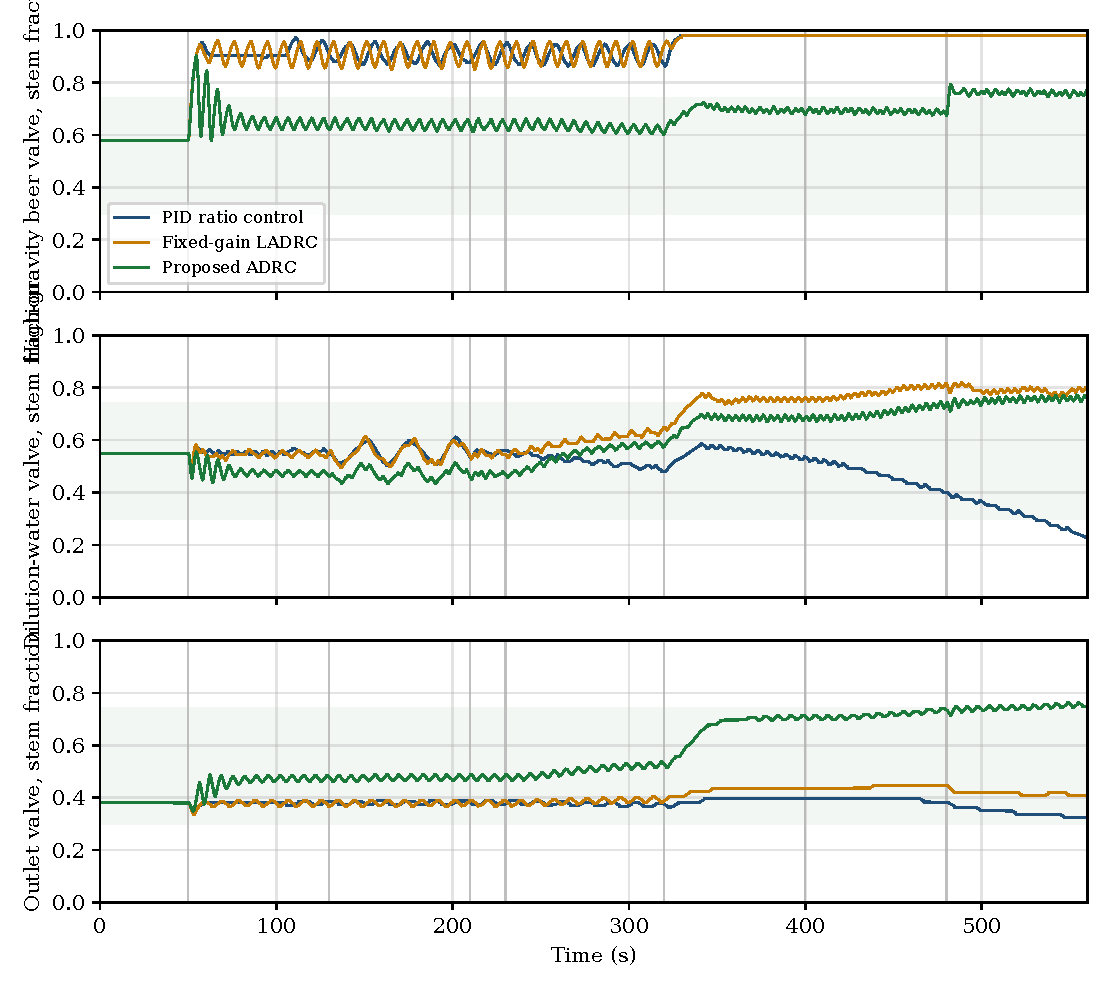
\includegraphics[width=\textwidth]{valves.pdf}
\caption{Stem fractions. The shaded band is the linear window $[0.30,0.74]$ in which the header bandwidth stays at its base value.}
\label{fig:valves}
\end{figure}

\subsection{Supply-pressure step}

On the window from \SI{50}{s} to \SI{130}{s} the extract integrals are $4.03$, $5.53$ and $3.36\ \degP\cdot\mathrm{s}$ for proportional--integral control, fixed-gain active disturbance rejection and the proposed pair. Settling to $\pm 0.05\degP$ takes \SI{72}{s} for proportional--integral control and \SI{46}{s} for the proposed pair. The fixed-gain observer does not stay inside the band before the next event. Its beer-flow integral on this window is \SI{14.0}{\cubic\metre\per\hour\second}, against \SI{12.8}{} for the proposed controller and \SI{7.7}{} for proportional--integral control. The proportional--integral flow loop is stiff at the old gain and so it recovers flow quickly, at the price of driving the beer stem to $0.91$. The proposed stem opens only to about $0.68$ and the header falls to \SI{1.85}{\barg}, which is the coordinator paying for that restraint with outlet travel of $1.02$ on the window, against $0.41$ and $0.12$ for the baselines.

Figure~\ref{fig:pressures} shows the supplies and the header. The proposed header setpoint leaves \SI{2.40}{\barg} within a few seconds of the step and settles near \SI{1.8}{\barg}. Both baselines hold \SI{2.40}{\barg}, as they were asked to. Holding it is what forces the beer valve up the installed curve of Figure~\ref{fig:installed}. The fixed-gain observer is slightly worse than proportional--integral control on this particular window because its $b_0$ is now too large for the reduced drop: the cancellation in \eqref{eq:ladrc-u} overstates the gain, the effective bandwidth falls, and the flow recovery is sluggish. The scheduled $b_{0,h}$ of \eqref{eq:b0h} removes that particular mistake. The remaining advantage of the proposed pair on the extract integral is the soft sensor, which trims $R$ from $\hat{P}$ while the baselines are still waiting for $P_{\mathrm{meas}}$.

\begin{figure}[htbp]
\centering
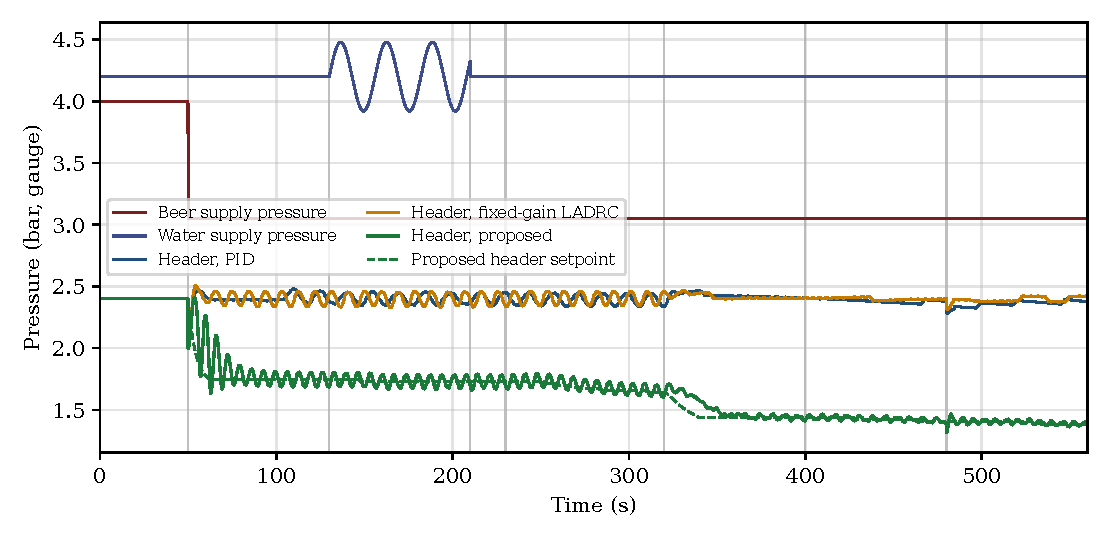
\includegraphics[width=\textwidth]{pressures.pdf}
\caption{Supply pressures and blend-header pressure. The proposed header setpoint is lowered after the beer-supply step so that the inlet valves keep their pressure drop.}
\label{fig:pressures}
\end{figure}

\subsection{Water-supply oscillation}

From \SI{130}{s} to \SI{210}{s} the water supply oscillates with amplitude \SI{0.28}{\barg}. Peak extract errors are $0.109$, $0.140$ and $0.086\degP$. Time spent outside $\pm 0.05\degP$ is \SI{30}{s}, \SI{32}{s} and \SI{7.8}{s}. The proposed beer-flow integral on the window is $4.89$, against $10.2$ for the fixed-gain observer and $6.62$ for proportional--integral control.

The oscillation is a measured disturbance. It enters $G_{ww}$ through $\Delta p_w$ on the sample it occurs. The water-loop $b_{0,w}$ therefore moves with the oscillation, lagged by the \SI{2.5}{s} gain filter, and the command partially anticipates the gain change. The fixed-gain observer must put the whole oscillation into $z_2$. It does reject it, which is why the extract error stays near a tenth of a degree rather than growing, but the rejection is late by a fraction of the observer bandwidth and the peak is the largest of the three. Proportional--integral control has no observer and rejects the oscillation by the integral state, with a peak between the other two. The header loop of the proposed controller moves as well, because the coordinator sees a changing water supply; the outlet travel on the window is $0.55$, and the stem plot shows a slow modulation rather than a copy of the \SI{26}{s} sine at high amplitude.

\subsection{Brand change}

The setpoint ramp from \SI{12.0}{\plato} to \SI{11.2}{\plato} occupies \SIrange{230}{255}{s}. The window used for the indices runs to \SI{320}{s}, so it includes the ramp and \SI{65}{s} of settling. Extract integrals are $76.2$, $39.6$ and $19.2\ \degP\cdot\mathrm{s}$. The proposed controller re-enters the $\pm 0.05\degP$ band \SI{89}{s} after the start of the window, that is about \SI{64}{s} after the ramp has finished. Neither baseline has settled when the throughput ramp begins.

This is the delay comparison. The required ratio change is from $0.338$ to $0.434$, a water-flow change of about \SI{0.72}{\cubic\metre\per\hour} at the pre-ramp beer flow. The soft sensor sees the extract move as soon as the water flow moves, and the extract bandwidth $0.12\ \si{\radian\per\second}$ finishes most of the change inside a minute. The analyser-based observer at $0.055\ \si{\radian\per\second}$, behind eleven seconds of delay, is still \SI{0.48}{\plato} high at \SI{280}{s} ($11.68$ against $11.20$). Proportional--integral control on the analyser is further behind, at $12.15$. Figure~\ref{fig:zoom} shows the three trajectories: the proposed extract follows the ramp with a lag of a few seconds, and the baselines follow a delayed and filtered copy of it.

The peak error of the proposed controller on this window is \SI{0.51}{\plato}, which occurs during the ramp itself, when the setpoint is moving faster than $\omega_{c,R}$ can follow. That peak is the cost of keeping the extract loop slower than the flow loops. Raising $\omega_{c,R}$ toward the flow bandwidth reduces the ramp lag and couples the extract loop into the water valve strongly enough to disturb the beer flow. The value in Table~\ref{tab:bw} is the compromise the build was tuned to, not the lowest integral achievable by a faster unstable loop.

\subsection{Throughput ramp under the reduced supply}

From \SI{320}{s} the beer-flow setpoint rises to \SI{9}{\cubic\metre\per\hour} while the beer supply is still \SI{3.05}{\barg}. This is the joint authority test. Beer-flow integrals on \SIrange{320}{400}{s} are $74.9$, $69.3$ and $4.83\ \si{\cubic\metre\per\hour\second}$. Extract integrals are $77.3$, $6.25$ and $3.68\ \degP\cdot\mathrm{s}$.

Figure~\ref{fig:flows} shows why the baseline flow integrals are large. Both baseline beer valves reach the open limit near $0.98$ and the delivered beer flow stays near \SI{8}{\cubic\metre\per\hour} or below. The fixed-gain extract controller then holds the extract reasonably well, at the wrong throughput: at \SI{360}{s} its extract is \SI{11.16}{\plato} against \SI{11.20}{\plato}, while its beer flow is \SI{7.96}{\cubic\metre\per\hour}. An extract specification that ignores the production rate would accept this. A blending specification does not, because the bright-beer tank fills slowly and the missing flow is not recovered later in the run. The proposed beer flow at the same instant is \SI{8.90}{\cubic\metre\per\hour} and at \SI{400}{s} it has reached the setpoint. The header is near \SI{1.45}{\barg} and the three stems are near $0.70$.

Proportional--integral control loses the extract as well as the flow on this window. With the beer valve saturated, the ratio $R$ no longer determines the extract, because $Q_h$ is stuck and the water loop is still trying to realise $R Q_h^\star$. The water flow and the beer flow drift apart and the extract at \SI{360}{s} is \SI{12.14}{\plato}, almost a degree above the new brand. The integral state of the extract loop cannot repair a ratio whose beer half is not a free input. This is the concrete form of the statement, in Section~\ref{sec:tech1}, that $z_2$ cannot invent travel beyond the stop.

\begin{figure}[htbp]
\centering
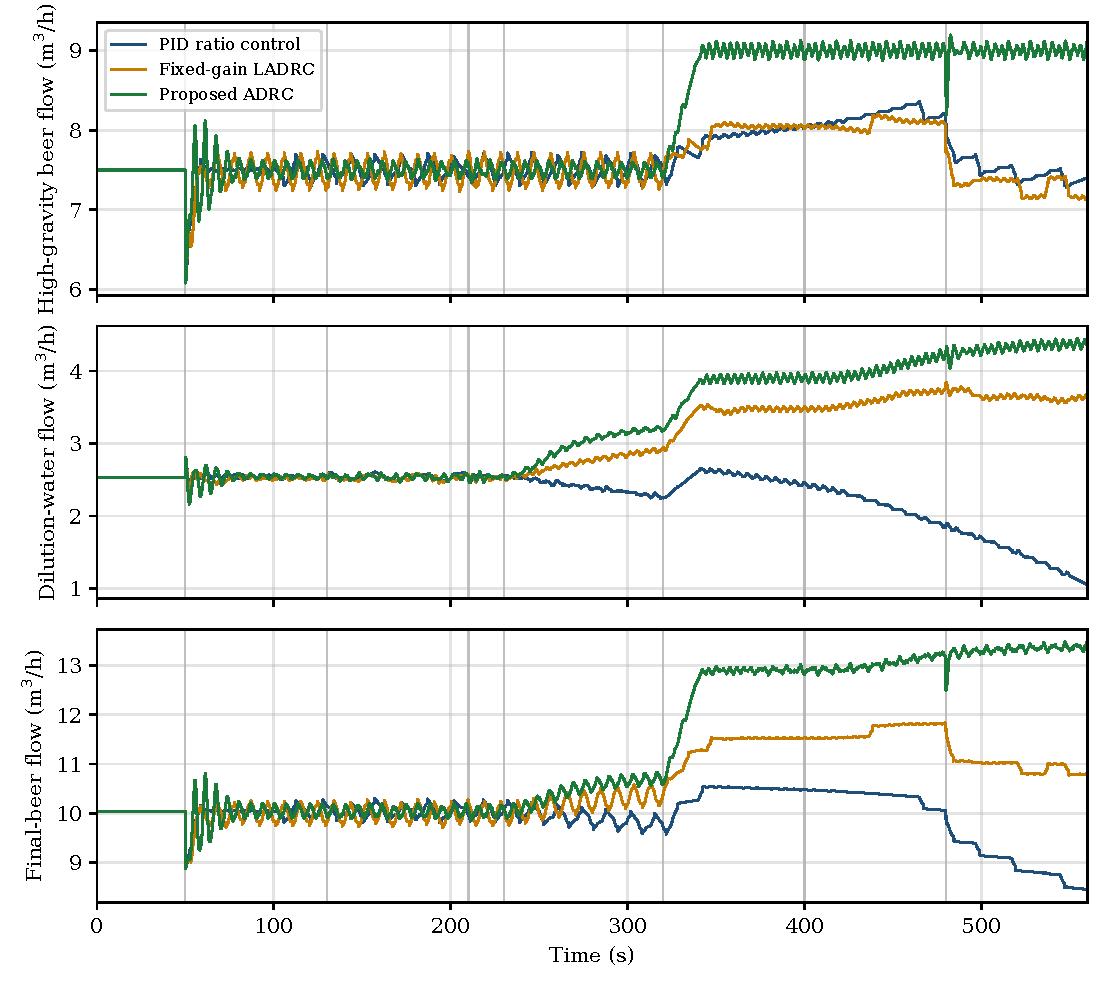
\includegraphics[width=\textwidth]{flows.pdf}
\caption{Volumetric flows. After \SI{320}{s} the beer-flow setpoint is \SI{9}{\cubic\metre\per\hour}. Only the proposed controller reaches it, because the header pressure has been lowered to keep the beer valve inside its travel.}
\label{fig:flows}
\end{figure}

\subsection{Unmeasured drift of the mother-beer extract}

From \SI{400}{s} to \SI{440}{s} the true $P_h$ rises from \SI{16.0}{\plato} to \SI{16.6}{\plato}. The controllers continue to use $16.0$ in any calculation that needs a mother-beer extract. On \SIrange{400}{480}{s} the extract integrals are $147$, $18.0$ and $17.4\ \degP\cdot\mathrm{s}$. The proportional--integral loop, already lost after the throughput ramp, integrates a large offset and finishes the window near \SI{13.3}{\plato}. The two observer-based extract loops both see the analyser. Their integrals are close. The proposed loop has a much smaller beer-flow integral on the same window, $3.99$ against $73.9$, because it is not sitting on the beer-valve stop while it trims water.

Figure~\ref{fig:softsensor} shows the proposed signals. The delayed analyser lags the true extract by about ten seconds. The corrected soft sensor $P_c$ lies between them and is what the extract observer tracks. The bias $b_P$ rises through the drift, as \eqref{eq:bias} requires, and does not run away: the innovation was built so that a bias larger than the true composition error is itself an innovation of the opposite sign. At \SI{450}{s} the true extract is \SI{11.53}{\plato} and at \SI{520}{s}, after the valve-wear transient, it is \SI{11.33}{\plato} against the setpoint \SI{11.20}{\plato}. The residual is the \SI{28}{s} bias lag still finishing its correction, not a frozen offset. A shorter $T_b$ reduces this residual and, in earlier builds of the same plant, produced an overshoot past the setpoint of several tenths of a degree. The recorded value is the slower, non-overshooting choice.

The fixed-gain extract loop ends the campaign closer to the setpoint on extract alone, at \SI{11.16}{\plato}. It does so at a beer flow of \SI{7.38}{\cubic\metre\per\hour}. The two numbers must be read together. A composition controller that is allowed to abandon the production rate has an easier composition problem, because it has an extra free input, the flow it chose not to deliver. The proposed controller is required to deliver both, and at \SI{520}{s} it delivers \SI{9.06}{\cubic\metre\per\hour} at \SI{11.33}{\plato}, with the bias still closing.

\begin{figure}[htbp]
\centering
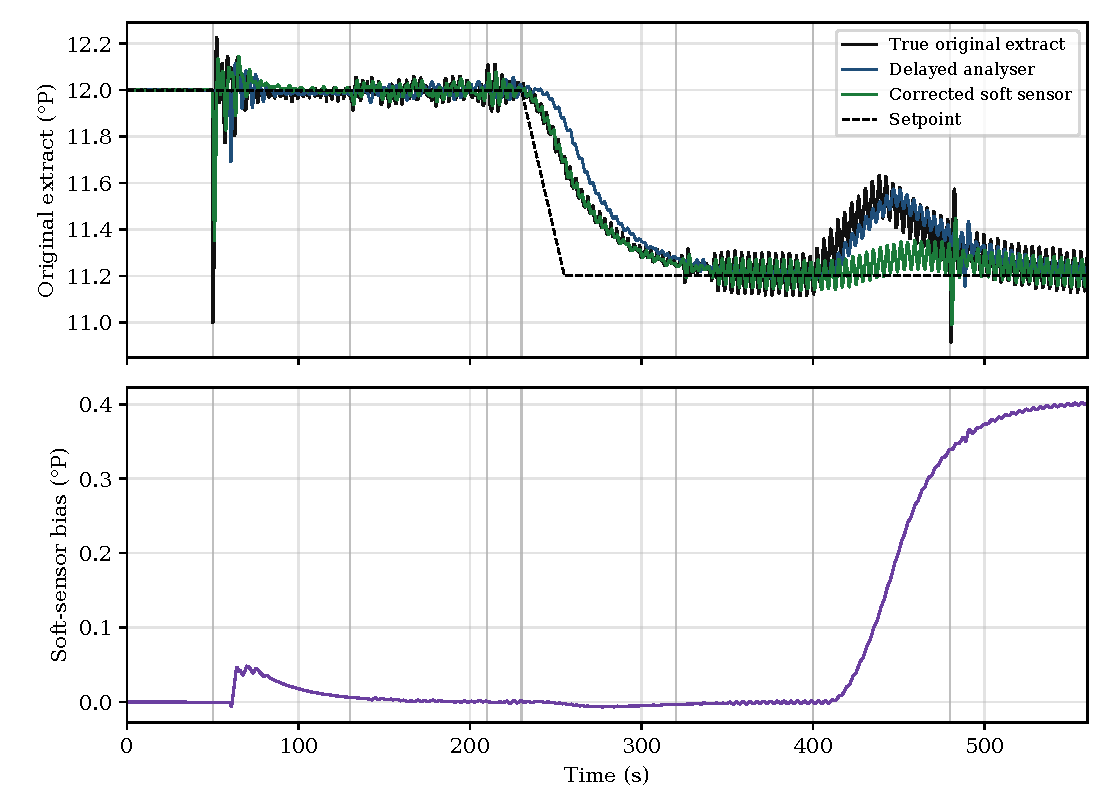
\includegraphics[width=\textwidth]{softsensor.pdf}
\caption{Proposed extract signals. The analyser lags the mix-point extract. The bias is the analyser correction applied to the mass-balance soft sensor.}
\label{fig:softsensor}
\end{figure}

\subsection{Loss of beer-valve capacity}

At \SI{480}{s} the beer $K_v$ falls by ten percent. Nothing in the controller is told. On \SIrange{480}{560}{s} the beer-flow integrals are $121$, $135$ and $4.60\ \si{\cubic\metre\per\hour\second}$. Extract integrals are $216$, $7.22$ and $6.05\ \degP\cdot\mathrm{s}$.

The installed-gain formula does not use $K_v$. It uses the flow that the weakened valve is actually passing. Within the \SI{2.5}{s} gain filter, $b_{0,h}$ falls and the beer command opens. The stem moves from about $0.70$ to $0.77$, the flow returns to \SI{9.06}{\cubic\metre\per\hour}, and the extract excursion peaks at \SI{0.38}{\plato}. The baseline beer valves are already at the stop, so a further loss of $K_v$ cannot be met by stem movement. Their beer-flow integrals on this window are the integrals of a flow that is stuck near \SI{7.3}{\cubic\metre\per\hour} against a setpoint of \SI{9}{\cubic\metre\per\hour}. Proportional--integral extract control drives the water valve shut in an attempt to raise the extract, and the extract reaches \SI{13.8}{\plato}. The fixed-gain extract observer, slower and delayed, holds the extract near the setpoint by a water flow that happens to match the reduced beer flow, and abandons the rate.

Figure~\ref{fig:bandwidth} shows the scheduled header bandwidth. It stays at the base value $0.20\ \si{\radian\per\second}$ for most of the campaign, because the coordinator keeps the stems inside the window that \eqref{eq:schedule} treats as acceptable. It rises only near the end, when the beer stem passes $0.74$ during the $K_v$ loss. The schedule is therefore a guard rather than a permanent retuning. A plant that needed the ceiling bandwidth for long intervals would be a plant whose outlet valve was too small for the requested flow, and the right response would be a larger $K_{v,b}$, not a faster observer. The outlet valve in Table~\ref{tab:design} was sized at stem $0.38$ precisely so that this guard would be enough.

\begin{figure}[htbp]
\centering
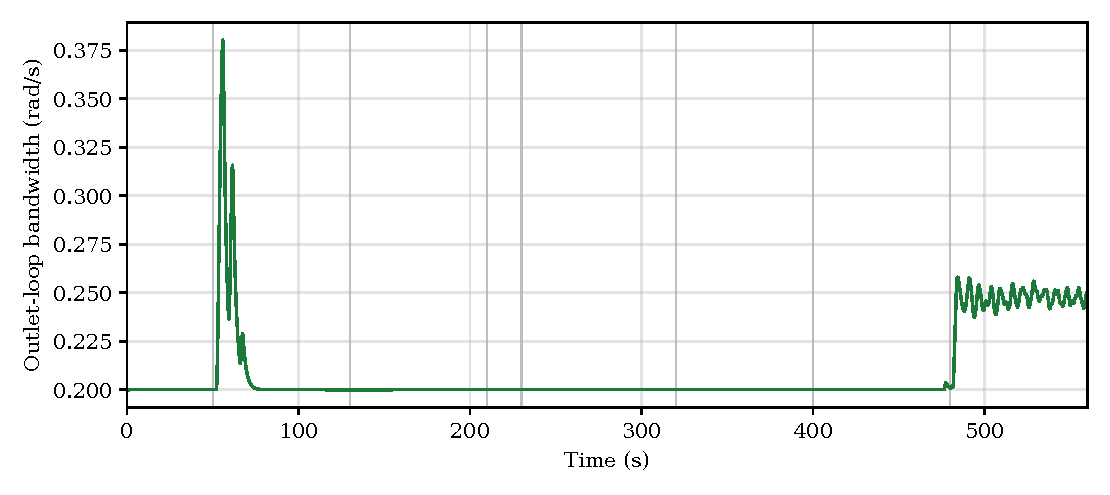
\includegraphics[width=\textwidth]{bandwidth.pdf}
\caption{Scheduled bandwidth of the outlet-valve controller. The base value is held while the inlet stems remain in the linear window.}
\label{fig:bandwidth}
\end{figure}

\subsection{Reading the baseline that looks quiet}

Proportional--integral control has the smallest valve travel in Table~\ref{tab:overall}. For the outlet valve the travel is $0.61$ over \SI{560}{s}. The stem plots show why. The outlet valve barely leaves its initial stick band, because the header error at a fixed setpoint of \SI{2.40}{\barg} stays near the threshold of the stick band for long intervals, and the inlet valves do the rejecting. Quiet travel here is an unused actuator. The extract and flow integrals are the cost of leaving it unused.

Fixed-gain active disturbance rejection is the stronger baseline, and on extract alone it is already an order of magnitude better than proportional--integral control. The bandwidth parameterisation, the consistent initial state and the observer anti-wind-up are doing the work Han and Gao described \cite{han2009pid,gao2003scaling,herbst2013simulative}. The campaign shows where that controller stops. It stops when the gain inside $b_0$ is wrong for a long time, and it stops when the only way to keep the gain right is to move a valve that the controller was not told to move. Those are the two gaps Chapter~\ref{ch:review} identified, and they are the two gaps the indices assign to the proposed pair: the flow integral falls from $316$ to $37.5$ because the header setpoint restores the drop, and the extract integral falls from $81.4$ to $52.4$ because the soft sensor removes the analyser delay from the brand change.

\subsection{What the estimation does not claim}

The plant is the design model, integrated at \SI{10}{ms}, with the disturbances of Table~\ref{tab:clock} and one noise draw. It does not include a pump curve, a bright-beer tank level, dissolved-oxygen dynamics, or the hysteresis of a valve that has been in service for years beyond the stick band used here \cite{choudhury2008stiction,jelali2010stiction}. A valve with a stick band of several percent would change the travel numbers and might force a lower $\omega_o$. The build acceptance tests of Section~\ref{sec:build} would still be the right first check on a factory skid: design-point flows, and the initial flow derivative after a small stem step, which confirms $b_0$.

The proportional--integral and fixed-gain observers were tuned by the same rules as the proposed loops, at the design point, and were not retuned against the later disturbances. Retuning the baselines at the low supply pressure would improve their behaviour at that pressure and worsen it at the design pressure. The proposed $b_0(t)$ is the retuning, done by the measurements, which is the comparison the technique is meant to win. A retuning that uses knowledge of the scenario clock would not be an admissible controller.

No index in this chapter is a flavour index. Stewart's review of high-gravity brewing records foam and ester differences that a correct original extract does not remove \cite{stewart2010highgravity,briggs2004brewing,boulton2001yeast}. The techniques keep the extract and the flow at the values the brand and the production plan specify. They do not enlarge the set of mother beers the brewery can ferment.

Within those limits the estimation is unambiguous. On a line with three linear valves, measured speeds and measured pressures, the pressure-manifold gain and the valve-authority setpoint are what keep the beer valve off the stop, and the mass-balance soft sensor with a delayed bias is what lets the extract loop run at the cascade bandwidth rather than at the delay bandwidth. The numerical values are those of Table~\ref{tab:overall}.

\subsection{Window table}

Table~\ref{tab:windows} repeats the indices at the resolution of Table~\ref{tab:clock}. It is the table a reader should use to check any sentence in this section. The steady window is the noise floor. Every later window is one disturbance, except that the supply pressure remains low after \SI{50}{s}, so the throughput window and the windows after it are joint tests with that low supply.

\begin{table}[htbp]
\centering
\caption{Extract IAE in $\degP\cdot\mathrm{s}$ and beer-flow IAE in \si{\cubic\metre\per\hour\second}, by window.}
\label{tab:windows}
\begin{tabular}{@{}lrrrrrr@{}}
\toprule
 & \multicolumn{3}{c}{Extract IAE} & \multicolumn{3}{c}{Beer-flow IAE} \\
\cmidrule(lr){2-4}\cmidrule(lr){5-7}
Window & PID & LADRC & Prop. & PID & LADRC & Prop. \\
\midrule
Steady & 0.005 & 0.005 & 0.005 & 0.007 & 0.007 & 0.007 \\
Pressure step & 4.03 & 5.53 & 3.36 & 7.71 & 14.0 & 12.8 \\
Water oscillation & 3.40 & 3.64 & 2.02 & 6.62 & 10.2 & 4.89 \\
Brand change & 76.2 & 39.6 & 19.2 & 8.73 & 11.3 & 5.08 \\
Throughput & 77.3 & 6.25 & 3.68 & 74.9 & 69.3 & 4.83 \\
Extract drift & 147 & 18.0 & 17.4 & 65.8 & 73.9 & 3.99 \\
Valve wear & 216 & 7.22 & 6.05 & 121 & 135 & 4.60 \\
\bottomrule
\end{tabular}
\end{table}

Two columns of this table carry the claim of the thesis. The beer-flow column from the throughput window onward is where valve authority is visible: the proposed integral stays near \SI{4}{\cubic\metre\per\hour\second} on an \SI{80}{s} window, which is a mean absolute error of about \SI{0.05}{\cubic\metre\per\hour}, while both baselines sit near \SI{70}{\cubic\metre\per\hour\second} or above, a mean error of about \SI{1}{\cubic\metre\per\hour} on a setpoint of \SI{9}{\cubic\metre\per\hour}. The extract column on the brand-change window is where the soft sensor is visible: the proposed integral is half the fixed-gain observer and a quarter of the proportional--integral loop. On the extract-drift window the two observers are close, and the proportional--integral loop has already been lost by the saturated beer valve. The techniques do different jobs, and the table shows both jobs rather than a single average that could hide one of them.

\subsection{Mean errors}

Dividing an integral by the length of the window gives a mean absolute error, which is easier to compare with the tolerance \SI{0.05}{\plato}. On the brand-change window of \SI{90}{s} the proposed mean absolute extract error is $19.2/90 = \SI{0.21}{\plato}$, most of it accumulated while the setpoint is still moving. On the pressure-step window of \SI{80}{s} it is $3.36/80 = \SI{0.042}{\plato}$, inside the tolerance on average, with the settling time of \SI{46}{s} saying that the first half of the window contains the excursion and the second half does not. The fixed-gain observer on that window averages $5.53/80 = \SI{0.069}{\plato}$ and does not settle. Proportional--integral control averages $4.03/80 = \SI{0.050}{\plato}$ and settles in \SI{72}{s}, with the beer stem already at $0.91$. Average extract error alone would rank proportional--integral control close to the proposed controller on the supply step. The stem and the later throughput window are what separate them: the proportional--integral loop has spent the authority the later ramp needed.

On the full run the proposed mean absolute extract error is $52.4/560 = \SI{0.094}{\plato}$ and the mean absolute beer-flow error is $37.5/560 = \SI{0.067}{\cubic\metre\per\hour}$. The fixed-gain observer's means are \SI{0.145}{\plato} and \SI{0.57}{\cubic\metre\per\hour}. The proportional--integral means are \SI{0.94}{\plato} and \SI{0.51}{\cubic\metre\per\hour}. The flow means of the two baselines are similar because both lose the beer valve for the same physical reason. Their extract means differ because the observer still trims water from the analyser and the proportional--integral loop, once the beer flow is stuck, trims water from a ratio that no longer describes the plant.

\subsection{Build parameters collected for reproduction}

A later estimation can reproduce the campaign from the following list, together with the equations of Chapter~\ref{ch:design}. Step \SI{10}{ms}. Positioner time constant \SI{2.4}{s}, stick release at stem error $0.014$, recapture at $0.005$. Command filter \SI{0.40}{s}. Measurement filter \SI{0.30}{s}. Gain filter \SI{2.5}{s}. Header-setpoint lag \SI{4}{s} outside a dead zone of \SI{0.04}{\barg}. Bias time \SI{28}{s}, bias limit $\pm 1.5\degP$. Pipe length \SI{14}{m}, analyser lag \SI{1.2}{s}. Noise standard deviations as in Section~\ref{sec:build}, generator seed fixed so that the three controllers share one draw. Flow limits on the stem command $[0.02,0.98]$, ratio limits $[0.08,0.85]$. Bandwidths as in Table~\ref{tab:bw}. Proportional--integral numbers as in Section~\ref{sec:build}. The header root is Brent's method on \eqref{eq:node}. Nothing in the campaign is filtered after the fact: the integrals use the true mix-point extract and the true beer flow at the controller sample rate.

\FloatBarrier
\typeout{END CHAPTER 3 ON PAGE \thepage}
